\documentclass[a4paper,12pt]{article} % добавить leqno в [] для нумерации слева
\usepackage[a4paper,top=1.3cm,bottom=2cm,left=1.5cm,right=1.5cm,marginparwidth=0.75cm]{geometry}
%%% Работа с русским языком
\usepackage{cmap}					% поиск в PDF
\usepackage[warn]{mathtext} 		% русские буквы в фомулах
\usepackage[T2A]{fontenc}			% кодировка
\usepackage[utf8]{inputenc}			% кодировка исходного текста
\usepackage[english,russian]{babel}	% локализация и переносы
\usepackage{physics}
\usepackage{multirow}
\usepackage{bm}
\usepackage{longtable}
\parindent = 1cm
%%% Нормальное размещение таблиц (писать [H] в окружении таблицы)
\usepackage{float}
\restylefloat{table}


\usepackage{graphicx}

\usepackage{wrapfig}
\usepackage{tabularx}

\usepackage{hyperref}
\usepackage[rgb]{xcolor}
\hypersetup{
	colorlinks=true,urlcolor=blue
}
\usepackage{pgfplots}
\pgfplotsset{compat=1.9}
%%% Дополнительная работа с математикой
\usepackage{amsmath,amsfonts,amssymb,amsthm,mathtools} % AMS
\usepackage{icomma} % "Умная" запятая: $0,2$ --- число, $0, 2$ --- перечисление

%% Номера формул
%\mathtoolsset{showonlyrefs=true} % Показывать номера только у тех формул, на которые есть \eqref{} в тексте,

%% Шрифты
\usepackage{euscript}	 % Шрифт Евклид
\usepackage{mathrsfs} % Красивый матшрифт

%% Свои команды
\DeclareMathOperator{\sgn}{\mathop{sgn}}

%% Перенос знаков в формулах (по Львовскому)
%\newcommand*{\hm}[1]{#1\nobreak\discretionary{}
%	{\hbox{$\mathsurround=0pt #1$}}{}}

\date{\today}

\begin{document}

\begin{titlepage}
	\centering
	\vspace{5cm}
	{\scshape\LARGE Московский физико-технический институт \par}
	\vspace{4cm}
	{\scshape\Large Лабораторная работа 4.2\par}
	\vspace{1cm}
	{\huge\bfseriesИзучение механизма окисления $LiFePO_4$ водными растворами пероксида водорода методом потенциометрии}
	\vspace{1cm}
	\vfill
\begin{flushright}
	{\large Б04-202}\par
	\vspace{0.3cm}
	{\LARGE Троянова Маргарита}\par
 {\LARGE Василега Анастасия}\par
\end{flushright}
	

	\vfill

% Bottom of the page
	2024 г.
\end{titlepage}
%\numberwithin{equation}{section}

\section{Введение}
\textbf{Цель работы:} В работе изучается механизм окисления водными растворами пероксида водорода микрочастиц $LiFePO_4$. По полученным экспериментальным данным строятся кинетические кривые изменения концентрации b проводится анализ по различным теоретическим моделям, в ходе которого определяются константы реакций при различных значениях $pH$.
\newline


\section{Теоретическое введение}\par 
\subsection{Современные химические источники тока}\par
$LiFePO_4$, один из реагентов изучаемой реакции, является одним из наиболее перспективных материалов используемых при создании литий-ионных аккумуляторов, являющихся вторичными химическими источниками тока(т.е. способные к циклированию).Основой работы ХИТ является химическая реакция взаимодействия окислителя и восстановителя. Один из основных критериев оценки ХИТ – удельная энергия – определяется стандартной свободной энергией токообразующей реакции.Наибольшей теоретической удельной энергией обладают системы с литиевым анодом. \par 
Использование металлического лития приводит к тому, что свежая поверхность лития покрывается в апротонных растворителях пассивной плёнкой, которая предотвращает электронный контакт с металлической основой. Это явление приводит к тому, что при каждом заряде часть лития выбывает из дальнейшей работы. Решение - литий-ионные аккумуляторы, в которых отсутствует металлический литий, а процессы разряда и заряда происходят за счёт переноса ионов лития с одного электрода на другой.\par 
В работе исследуется кинетика процесса деинтеркаляция литий железа фосфата(на положительном электроде). Это актуально, так как необходимо оптимизировать состав химических добавок для улучшения его электронной проводимости.\par  
При исследовании процесса делитирования $LiFePO_4$ при окислении его суспензий в растворах пероксида водорода. Обнаружено возникновение периодических колебаний значений рН и окислительно-восстановительного потенциала .
В слабощелочной среде с $pH>8$ происходит выделение ионов лития, а отрицательный заряд компенсируется за счёт восстановления ионов железа.Уравнение реакции имеет вид:$$2LiFePO_4+H_2O_2 \rightarrow 2FePO_4 + 2LiOH$$\par 
В кислой среде можно моделировать процессы, происходящие при зарядке аккумулятора:
$$LiFePO_4 - xe^- \rightarrow Li_{(1-x)}FePO_4 + xLi^+$$\par 
\subsection{Механизм реакции}
Процесс окисления $LiFePO_4$ раствором $H_2O_2$ относится к гетерогенным гетерофазным некаталитическим реакциям. В этом случае реагенты находятся в разном фазовом состоянии, продукты реакции также могут находиться в любом фазовом состоянии. \par 
Их особенность состоит в том, что процесс можно разделить на несколько стадий:конвективный подход реагента, адсорбция на поверхность, диффузия через пористый слой продукта реакции к ядру, химическая реакция на поверхности, диффузия по поверхности поры от ядра. Основной задачей гетерогенной кинетики является определение лимитирующей стадии процесса и скорости всего процесса.\par 
В твердофазной реакции оценку лимитирующей стадии производят по диапазону энергии активации(области реагирования. Если лимитирующей является химическая реакция(кинетическая область реагирования) - $E_a > 40$кДж/моль. Если диффузия(диффузионная область реагирования) - $E_a < 10$ кДж/моль.\par
Характерной особенностью этого процесса рассматриваемой реакции является локализация реакционной зоны на поверхности раздела фаз твёрдого реагента –  $LiFePO_4$ и твёрдого продукта реакции – $FePO_4$.\par 
Это топохимическая реакция, т.е. зона реагирования может менять локацию в процессе реакции. В топохимических реакциях ионы лишены большой подвижности, поэтому значение имеет сама структура кристалла. Также продук реакции сохраняет форму кристаллов исходного вещества.\par
\subsection{Уравнение Ерофева}
Кинетика хорошо описывается уравнением Ерофеева:
\begin{equation}
    \alpha = 1- e^{-\int p dt},
\end{equation}
где p- вероятность реагирования, $\alpha$ - доля прореагировавшего вещества к моменту времени t. \par 
\begin{equation}
    \alpha = 1- e^{-kt^n},
\end{equation}
Обобщённо- кинетическое уравнение Ерофеева-Колмогорова, где n - число последовательных стадий при образовании устойчивого начального центра новой фазы, плюс постоянное число, характеризующее форму зародыша, и равное 3 при образовании сферического зародыша, 2 – цилиндрического и 1 – плоского. Если n>1, то процесс находится в кинетической области, при n<1 - процесс в диффузионной области. Для анализа данных строят график в линеаризованных координатах $ln(-ln(1-\alpha))$ от $lnt$. Тангенс угла наклона - n, пересечение - $lnk$.\par 
\subsection{Закон Авраами}Другой закон зародышеобразования был предложен Авраами:
\begin{equation}
    N(t) = N_0[1-exp(-kt^n)],
\end{equation}
где $N_0$ - число потенциальных центров зародышеобразования, имеющих равную вероятность превратиться в растущий зародыш; $N(t)$ -  реальное число зародышей, образовавшееся к моменту времени t.\par 
Выражение для скорости изменения степени превращения вещества ($\alpha$) в продукт новой фазы имеет вид(справедливо при малых {$\alpha$}:
\begin{equation}
    \alpha(t) =\frac{8\pi \rho N_0\nu}{k_1^3m_0}[e^{-k_1t}-1+k_1t-\frac{(k_1t)^2}{2}+\frac{(k_1t)^3}{6}]
\end{equation}
\subsection{Уравнение Ленгмюра}\par 
Эту реакцию можно рассматривать как реакцию ионного обмена между $Li^+$ и $Fe^3+$. При этом значения сорбционной ёмкости зависят от времени сорбции. Изотермы катионного обмена описываются уравнением Ленгмюра:
\begin{equation}
    A_t = A_mkC_p\frac{1}{1+kC_p},
\end{equation}
где K - константа Ленгмюра, $C_p$ -равновесная концентрация сорбата, $A_t$ - текущее значение сорбционной ёмкости, $A_m$ - величина сорбционной емкости в равновесных условиях. .\par 
При предположении, что количество реагирующих центров в сорбенте зависит не только от концентрации сорбата в растворе C, о и от времени сорбции. Также десорбция принята зависимой от концентрации сорбата в растворе и относительной величины ёмкости сорбента:
\begin{equation}
    A_t = k_1Ct(1-\frac{A_t}{A_m})\ \ \ A_t = k_2C\frac{A_t}{A_m}\ \ \ \frac{1}{A_t} = \frac{1}{A_m} + \frac{1}{ktA_m},
\end{equation}
где k -константа скорости реакции ионного обмена($c^{-1}$), определяется из угла наклона $1/A_t(1/t)$.\par 
\subsection{Потенциометрический анализ}Поскольку в эксперименте для определения концентрации протонов и ионов лития используется метод потенциометрии, рассмотрим его основные теоретические положения. Метод потенциометрии основан на измерении напряжения на электродах ячейки в отсутствие тока. При этом, один из электродов является индикаторным электродом, а другой – электродом сравнения. Измеряемое вольтметром напряжение на электродах ячейки в соответствии с уравнением Нернста в общем случае равно: 
\begin{equation}
    E_{eq} = E_0 +\frac{RT}{zF}ln\frac{a_{ox}}{a_{red}}
\end{equation}
\subsection{Стеклянный электрод для измерения $pH$}
Чувствительным элементом стеклянного электрода является шарик диаметром 15-20 мм с толщиной стенок 0,06-0,1 мм, изготовленной из стекла особого состава, расположенной на конце стеклянной трубки . Внутри шарика – раствор с определенным значением рН , в который погружен хлорсеребряный электрод сравнения. Перед работой стеклянный электрод некоторое время выдерживают в 0,1М $HCl$. При этом ионы Н+ из раствора обмениваются на ионы Na+ из мембраны, и в системе устанавливается равновесие.Если подготовленный таким образом электрод опустить в анализируемый раствор, содержащий ионы $H^+$, установится ионообменное равновесие между раствором и внешней поверхностью мембраны, приводящее к возникновению потенциала Нернста –  Е1.
\subsection{Селективные электроды}\par 
Изменяя химический состав стекла, получают ионоселективные электроды для других одновалентных ионов. Ключевым этапом подготовки электродов к работе является процедура выдерживания ионоселективного электрода в растворе соли соответствующего элемента. 
\section{Оборудование и материалы}
\begin{enumerate}
    \itemИономер И-160М
\item $рН$-метр $рН$150М
\item Магнитная мешалка
\item Аналитические весы
\item Секундомер
\item Микрошпатель для порошков
\item Мерный цилиндр или мерная колба объемом 250 мл
\item Пластиковая емкость с крышкой объёмом 1 л.
\item Стеклянный $рН$ - чувствительный электрод
\item 	Стеклянный литий - селективный электрод
\item Хлорсеребряный электрод сравнения
\item Дозатор переменного объема 100-1000 мкл (2 шт.)
\item Пластиковый наконечник с капилляром
\item Стеклянный стакан объемом 250 (2 шт.)
\item Образец $LiFePO_4$
\item Растворы хлорида лития (1 мМ и 100 мМ)
\item Раствор пероксида водорода (15 М)
\item Гидрофосфат калия ($К_2НРО_4$)
\item Раствор соляной кислоты (3 М)
\item Дистиллированная вода

\end{enumerate}
\section{Результаты и обсуждения}\par 

Задачей лабораторной работы является исследование влияния $рН$ растворов $Н_2О_2$ на скорость окисления $LiFePO_4$, с целью изучения механизма данного процесса. Для этого предлагается проводить эту реакцию в буферных растворах $К_2НРО_4$ с концентрацией 5-10 мМ и значениями $рН$ в диапазоне 7-9 в режиме $рН$-статирования, реализуемого с помощью постепенного добавления раствора соляной кислоты.
\begin{enumerate}
    \item Сначала провели калибровку стеклянного литий - селективного электрода, а с помощью буферного раствора провели калибровку pH-метра. 
    \item Для приготовления 1л 5мМ раствора $K_2HPO_4$ взвесили m = 1,14 г вещества.
    \item Отмерили 250 мм раствора $K_2HPO_4$ и перелили в стакан
    \item Поставили стакан с раствором $K_2HPO_4$ на магнитную мешалку,опустили $pH$ метр и литий-селективный электрод; с помощью дозатора с капилляром с $HCl$ довели значение $pH$ до 9.
    \item Добавили 0,4 г $LiFePO_4$ и 1000 мкл 6,3 М раствора $H_2O_2$.
    \item В течение 15-20 минут поддерживали $pH$ постоянным, прибавляя $HCl$ и через каждую минуту записывали значение концентрации ионов лития и объёма добавленной кислоты.
    \item Аналогичные измерения провели для растворов с $pH$=8,5/8,0/6,7.Результаты представлены в таблице в приложении. Концентрация $HCl$ была рассчитана исходя из того, что добавляемый раствор $HCl$ был 2М на 250 мл.
    \item Построили кинетические кривые, зависимость концентраций ионов лития и хлорида лития при окислении.
    \begin{figure}[H]
	\center{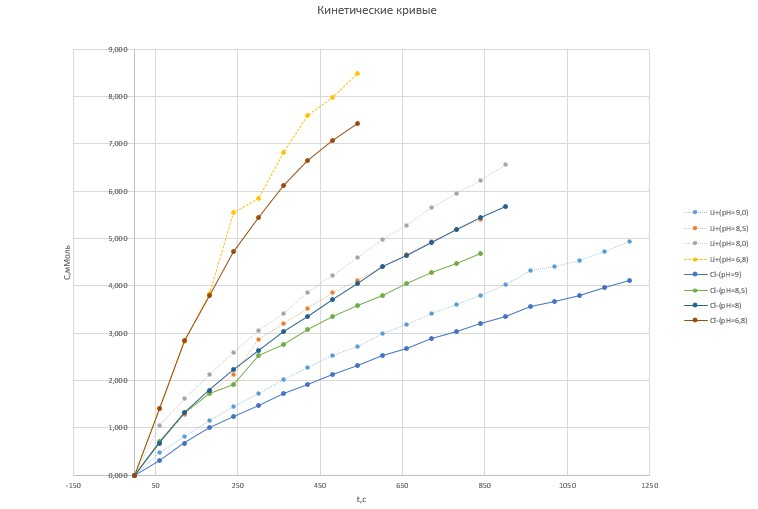
\includegraphics[scale=0.8]{1.jpg}}
	\caption{\centering Кинетические кривые }
	\label{pic:5}
\end{figure}
В каждом случае график кинетической кривой ионов лития был выше, чем аналогичный с хлорид ионами, но не намного. Наблюдается рост скорости реакции при увеличении pH. Это можно объяснить тем, что в более кислой среде при окислении железа до +3 увеличение числа протонов способствует усилению электростатического взаимодействия между их положительным зарядом и отрицательным зарядом электрона железа(которое может находится в глубине кристаллической решётки вещества, что изначально затрудняет доступ). Тем самым, "оторвать" электрон у железа легче, что способствует ускорению реакции. В начале реакции самый большой рост из-за высокой скорости зародышеобразования. Затем отдельные центры реакции(на границе 2ух твёрдых фаз продукта и реагента) создают сплошной фронт, продвигающийся вглубь твёрдой фазы. Мы не находим перегиба на кинетической кривой, 
что свидетельствует о постоянном замедлении процесса реакции.\par 
\itemОпределим степень делитирования как $\alpha = \frac{C}{C_0}$, где $C$-концентрация $Li^+$(мМоль) на 9 минуте, $C_0$ = 0,01М. Значения представлены в таблице 1. Степень делитирования увеличивается более чем в 3 раза при возрастании кислотности.

\begin{table}[H]
	\center{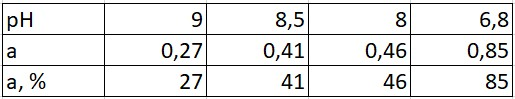
\includegraphics[scale=0.5]{2.jpg}}
	\caption{\centering Степень делитирования }
    \label{tab:my table} 
    \end{table}

\item Провели анализ экспериментальных данных по уравнению Ерофеева-Колмогорова, где  $\alpha = \frac{C}{C_0}$ - доля прореагировавшего вещества к моменту времени t.График в координатах $ln(-ln(1-\alpha))(lnt):$
 \begin{figure}[H]
	\center{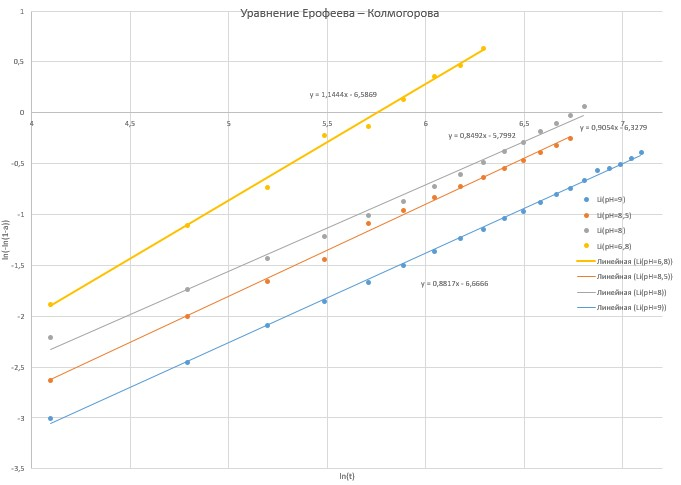
\includegraphics[scale=0.8]{3.jpg}}
	\caption{\centering Уравнение Ерофеева-Колмогорова }
	\label{pic:5}
\end{figure}
Видно, что графики аппроксимируются прямой(хуже всего ложится при pH=8). Так как n - тангенс угла наклона прямой, а пеесечение с осью ординат $lnk$. Сведём результат в таблицу:
\begin{table}[H]
	\center{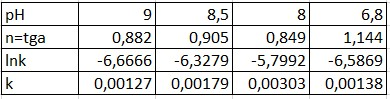
\includegraphics[scale=0.5]{4.jpg}}
	\caption{\centering Константы скорости и коэффициент n }
    \label{tab:my table} 
    \end{table}

Если принимать, что точки хорошо аппроксимируются прямыми, то т.к. коэффициент n<1 в первых 3-х случаях(т.е. в щелочной среде), то можно сказать, что лимитирующая стадия диффузионная, т.е. или подвод реагента к частице или диффузия вглубь частицы через поры. Тогда как n при большем $pH$ превышает 1, следовательно процесс переходит в кинетическую область.
\item Определим константу скорости исходя из уравнения (6). Для этого построим зависимость обратной концентрации ионов лития от обратной величины времени:
\begin{figure}[H]
	\center{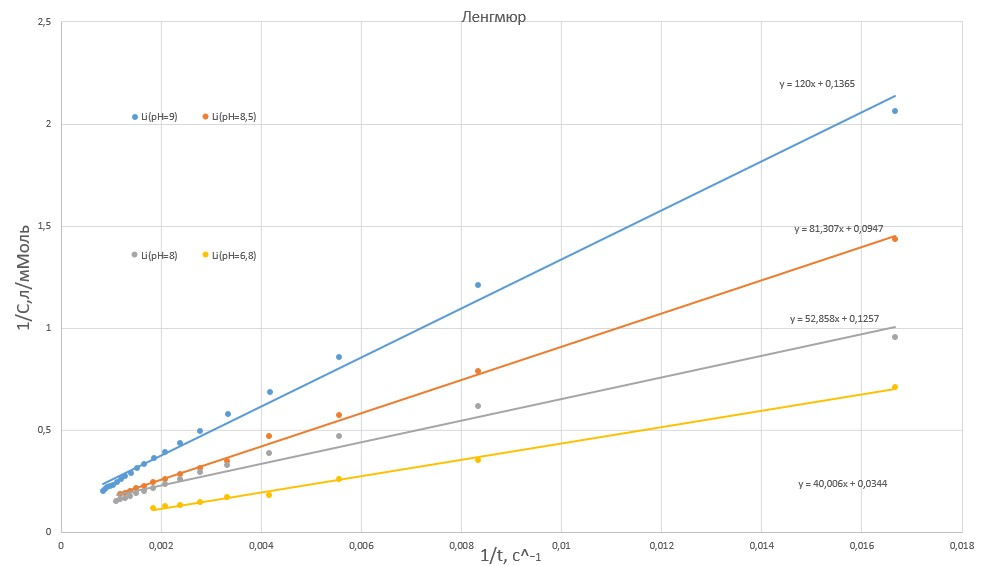
\includegraphics[scale=0.8]{5.jpg}}
	\caption{\centering Уравнение Ленгмюра }
	\label{pic:5}
\end{figure}
Результаты тоже хорошо аппроксимируются прямой. Получа зависимость $y=ax+b$, где $a=1/A_m,\ \ \ a = b/K$, посчитаем $K=b/а$ и сведём результат в таблицу, сравнив с прошлым:
\begin{table}[H]
	\center{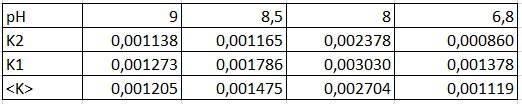
\includegraphics[scale=0.5]{6.jpg}}
	\caption{\centering Константы скорости и коэффициент n по уравнению Ленгмюра}
    \label{tab:my table} 
    \end{table}
Константы совпадают по порядку с посчитанными в предыдущем случае, но, кажется, что измерение при $pH$=8,0 ошибочно и вносит существенную погрешность.
\item Построим зависимость $LgK$ от $LgH$:
\begin{figure}[H]
	\center{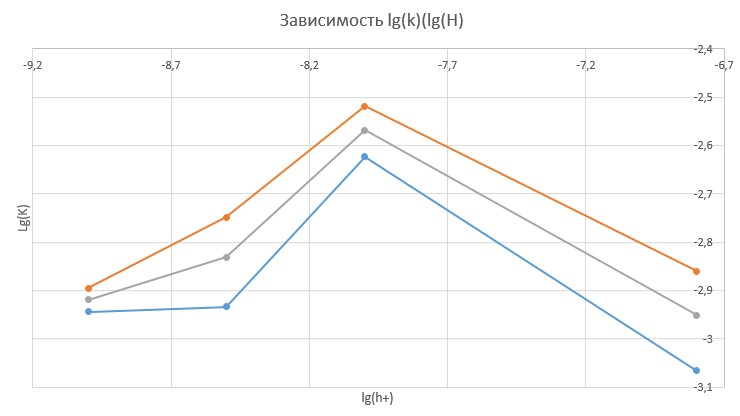
\includegraphics[scale=0.8]{7.jpg}}
	\caption{\centering Зависимость константы скорости от концентрации протонов }
	\label{pic:5}
\end{figure}
Сначала(в щелочной среде) константа скорости возрастала, а в кислой среде пошла на спад. Может, это из-за того, что вкислой среде реакция очень быстро завершилась. Хотя, не кажется, что можно делать какой-то вывод по этим 4-м точкам, учитывая, что в ходе обработки данных выпадала 3-яя точка(pH=8). Вполне возможно это произошло из-за неточной нормировки концентрации ионов лития.
\end{enumerate}
\section{Выводы}Изучена кинетика химического окисления 
$LiFePO4$ в водной щелочной среде с  
контролем ионов лития в растворе для определения кинетических характеристик процесса делитирования в зависимости от кислотности среды.
В  рамках представлений о  топохимических 
и диффузионно-контролируемых реакциях проанализированы кинетические кривые делитирования $LiFePO4$ . Сделан вывод о переносе через слой продукта 
реакции как лимитирующей стадии в щелочной среде. Используя 2 модели механизма реакции, посчитаны константы скорости, свопадающие по порядку.


\end{document}
